\documentclass[tikz, border=10pt]{standalone}
\usetikzlibrary{arrows.meta,positioning,shapes,snakes}

\tikzset{%
  >={Latex[width=2mm,length=2mm]},
  % Specifications for style of nodes:
            base/.style = {rectangle, rounded corners, draw=black,
                           minimum width=4cm, minimum height=1cm,
                           text centered, font=\sffamily},
  activityStarts/.style = {base, fill=blue!30},
       startstop/.style = {base, fill=red!30},
    activityRuns/.style = {base, fill=green!30},
         process/.style = {base, minimum width=2.5cm, fill=orange!15,font=\ttfamily},
}

\begin{document}
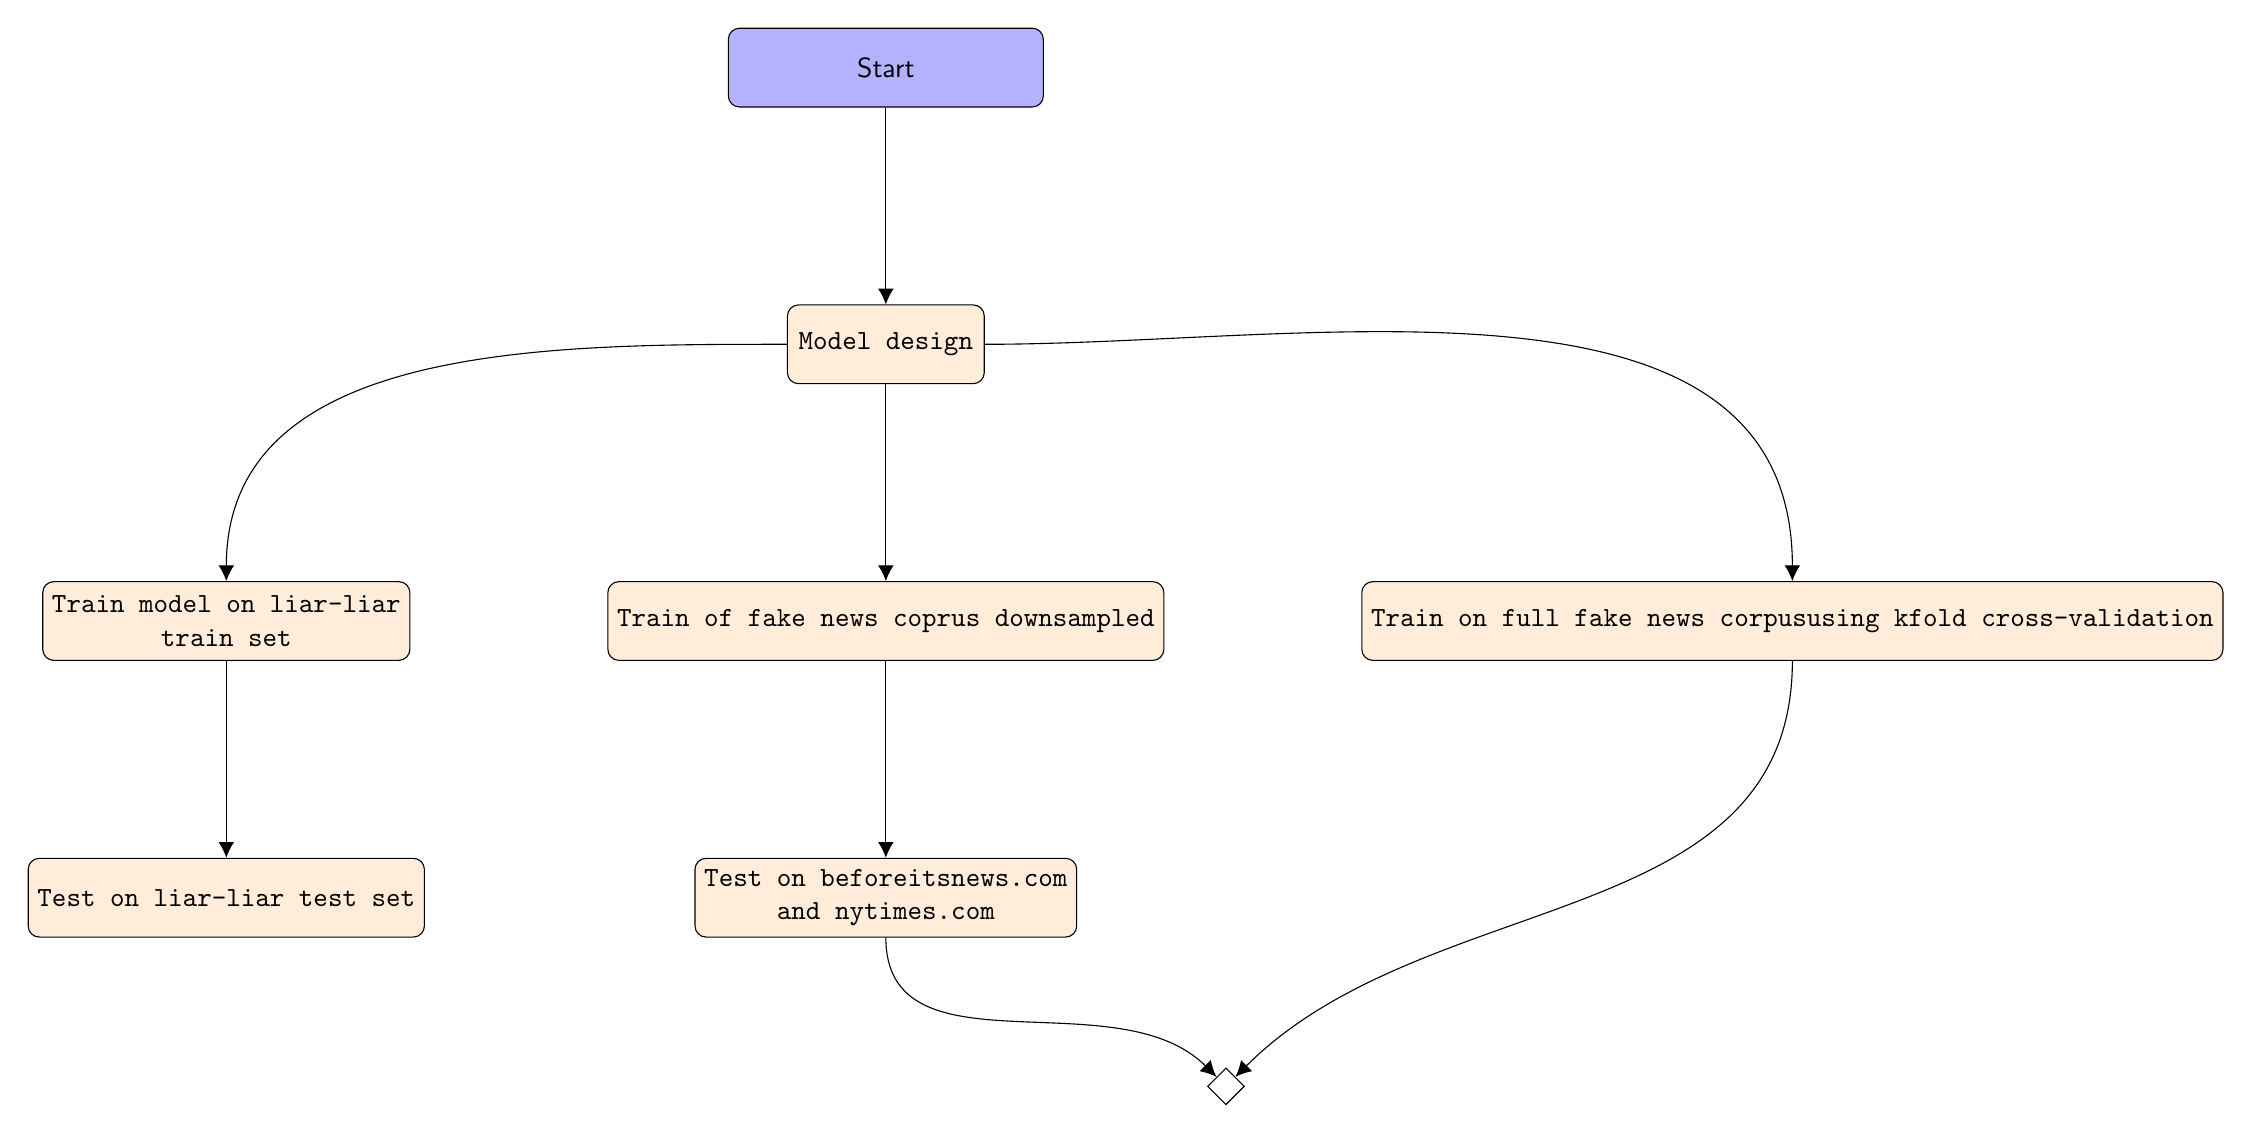
\begin{tikzpicture}[node distance=2.5cm,
    every node/.style={fill=white, font=\sffamily}, auto]

    \node (start) [activityStarts] {Start};
    \node (design) [process, below = of start] {Model design} edge [<-] (start);
    \node (downsampled) [process, below = of design, node distance=5cm] {Train of fake news coprus downsampled} edge [<-] (design);
    \node (downsampled_test) [process, below = of downsampled, align=center] {Test on beforeitsnews.com \\ and nytimes.com} edge [<-] (downsampled);


    \node (liar-liar) [process,left = of downsampled, align=center] {Train model on liar-liar \\ train set};
    \node (liar-liar-test) [process, below = of liar-liar, align=center] {Test on liar-liar test set};
    \draw [->] (liar-liar) to  (liar-liar-test);
  

    \node (not_downsampled) [process, right = of downsampled] {Train on full fake news corpus \\ using kfold cross-validation};
    \node (fake-corpus-test) [diamond, below right = of downsampled_test, draw=black] {};

    \draw [->] (downsampled_test) to [out = 270, in = 135] (fake-corpus-test);
    \draw [->] (not_downsampled) to [out = 270, in = 45] (fake-corpus-test);

    \draw [->] (design) to [out=180, in=90] (liar-liar);
    \draw [->] (design) to [out=0, in=90] (not_downsampled);
\end{tikzpicture}
\end{document}

